\documentclass[aspectratio=169,11pt]{beamer}

\usetheme{Madrid}
\usecolortheme{default}
\usefonttheme{professionalfonts}
\setbeamertemplate{navigation symbols}{}
\setbeamertemplate{footline}[frame number]

\usepackage{amsmath, amssymb, booktabs, graphicx}
\graphicspath{{../../assets/figures/}{assets/figures/}}

\title{Minimum Wages and Wage Regulations}
\subtitle{Labor II --- Week 7}
\author{Teaching deck draft}
\date{}

\begin{document}

\begin{frame}
  \titlepage
\end{frame}

\begin{frame}{Central question and course repositioning}
\begin{itemize}
    \item What do wage floors and related wage laws do to wages, employment, hours, turnover, and reallocation?
    \item Week 7 is the policy sequel to Week 6: minimum wages test whether the competitive benchmark is the right organizing model.
    \item Week 8 will then ask how legal floors interact with unions, bargaining, and worker voice.
\end{itemize}
\end{frame}

\begin{frame}{Week 6 to Week 7 bridge}
\begin{itemize}
    \item Week 6: firms may face finite labor supply to the firm.
    \item Week 7: if firms have wage-setting power, a wage floor need not reduce employment one-for-one.
    \item The policy question is not only ``do jobs fall?'' but which margins adjust and under what institutions.
\end{itemize}
\end{frame}

\begin{frame}{Competitive versus monopsony predictions}
\[
N_t = D(w_t),
\qquad
w_t = \max\{w_t^\ast, \bar w_t\}
\]

\[
N(\bar w) = S_f(\bar w),
\qquad
 \text{for } w^m < \bar w < w^c
\]

\begin{itemize}
    \item Competitive benchmark: binding floor raises wages and lowers employment.
    \item Monopsony benchmark: a floor can raise wages with small employment losses or even higher employment over a range.
    \item The sign of the employment effect is empirical, but the mechanism is not theory-free.
\end{itemize}
\end{frame}

\begin{frame}{Theory picture}
\begin{center}
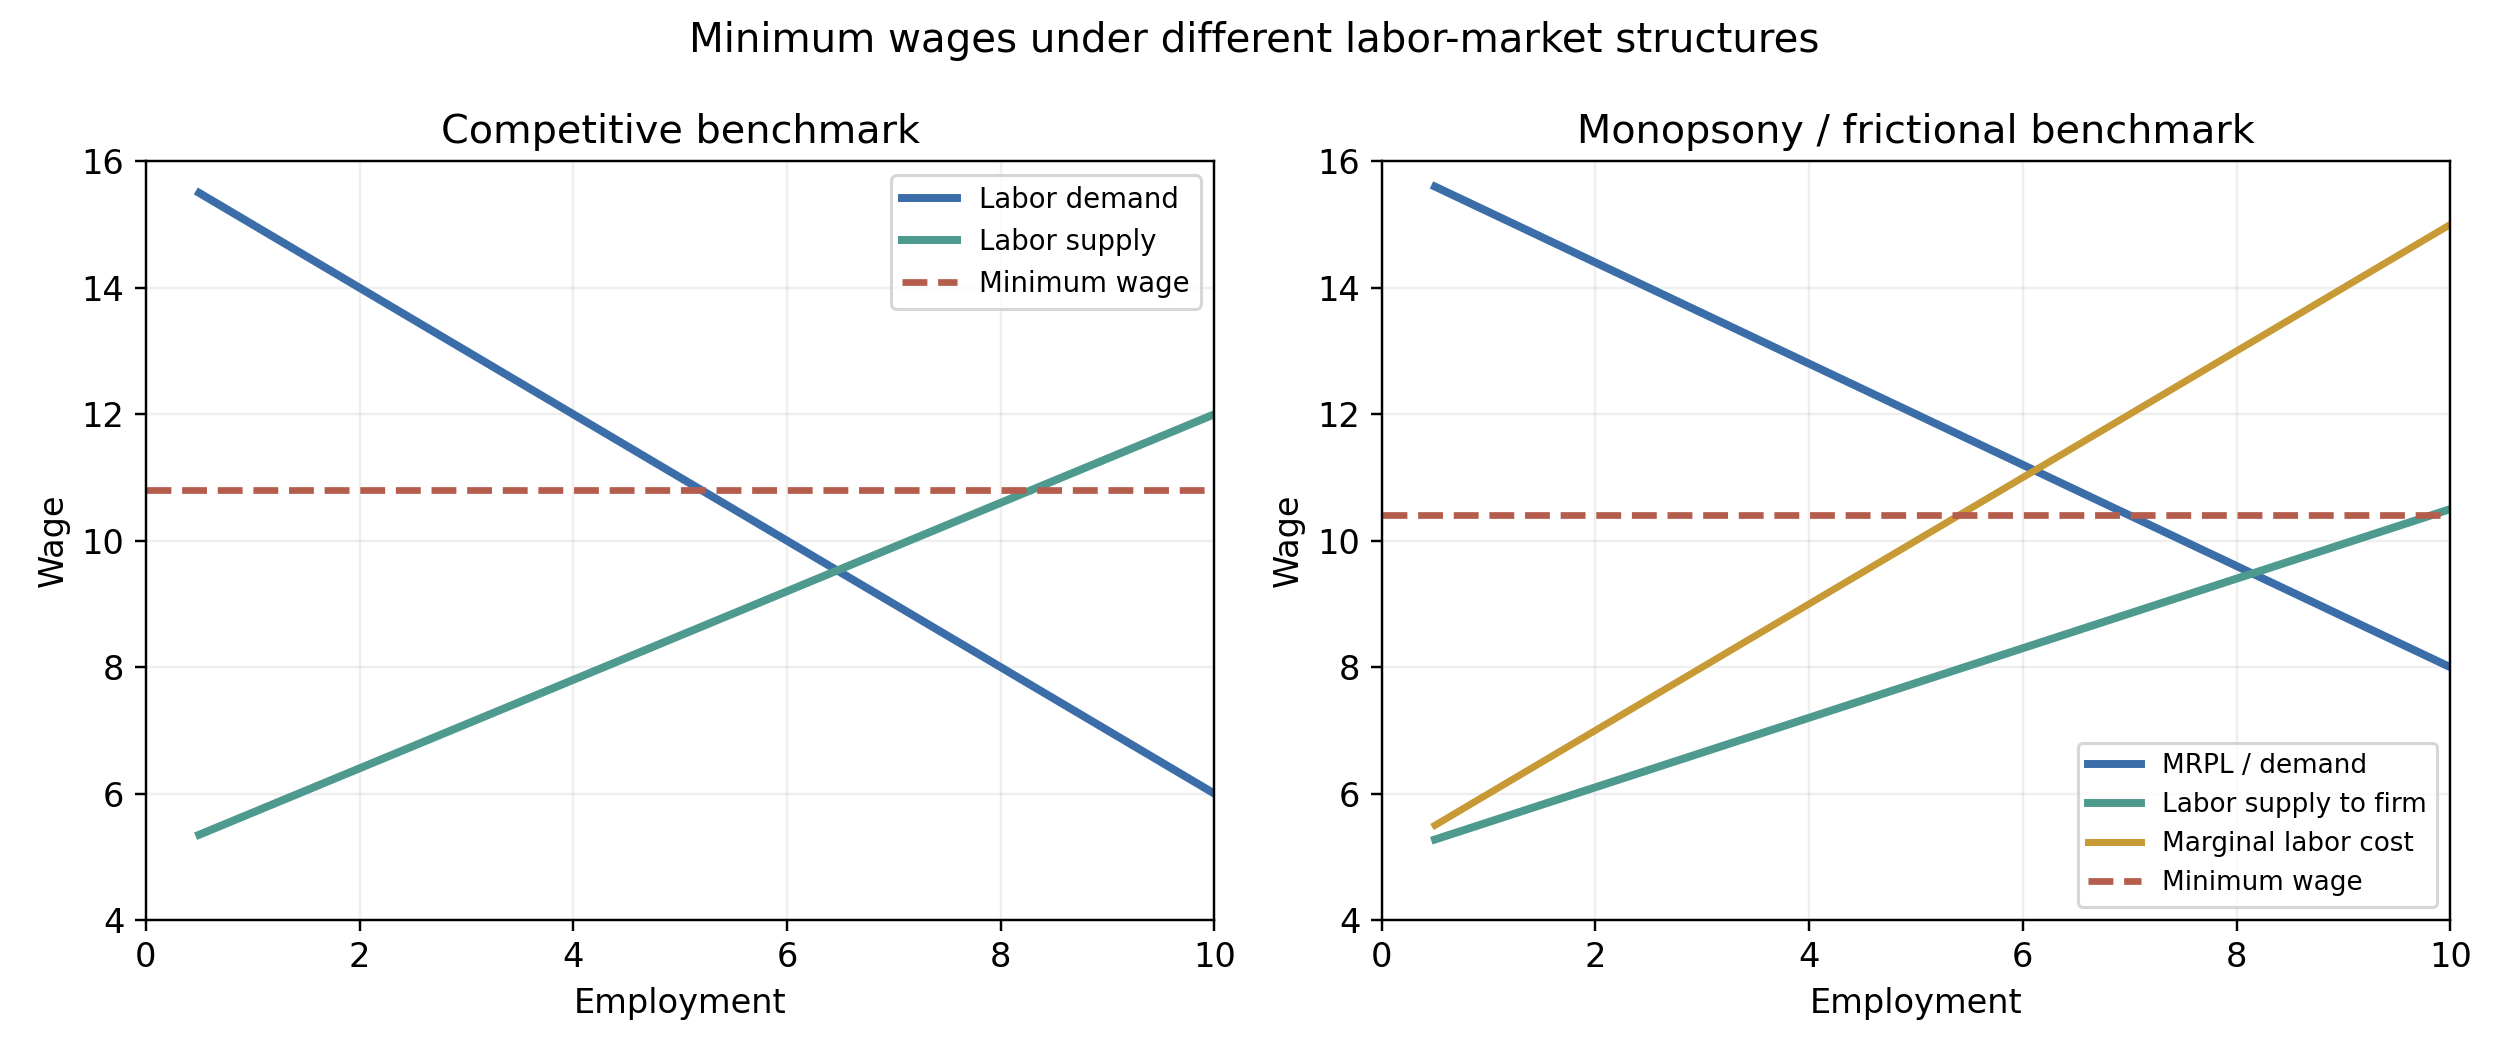
\includegraphics[height=0.72\textheight]{07-competitive-vs-monopsony-minimum-wage.png}
\end{center}
\end{frame}

\begin{frame}{What exactly is the employment debate?}
\begin{itemize}
    \item Card-Krueger turned the issue into a design problem with a treated sector and explicit comparison group.
    \item Neumark-Wascher emphasized broader panels, trend heterogeneity, and sensitivity to specification.
    \item Dube-Lester-Reich tightened local comparisons with border counties.
    \item Cengiz-Dube-Lindner-Zipperer changed the outcome object to low-wage jobs around the threshold.
\end{itemize}
\end{frame}

\begin{frame}{Employment-debate landscape}
\begin{center}
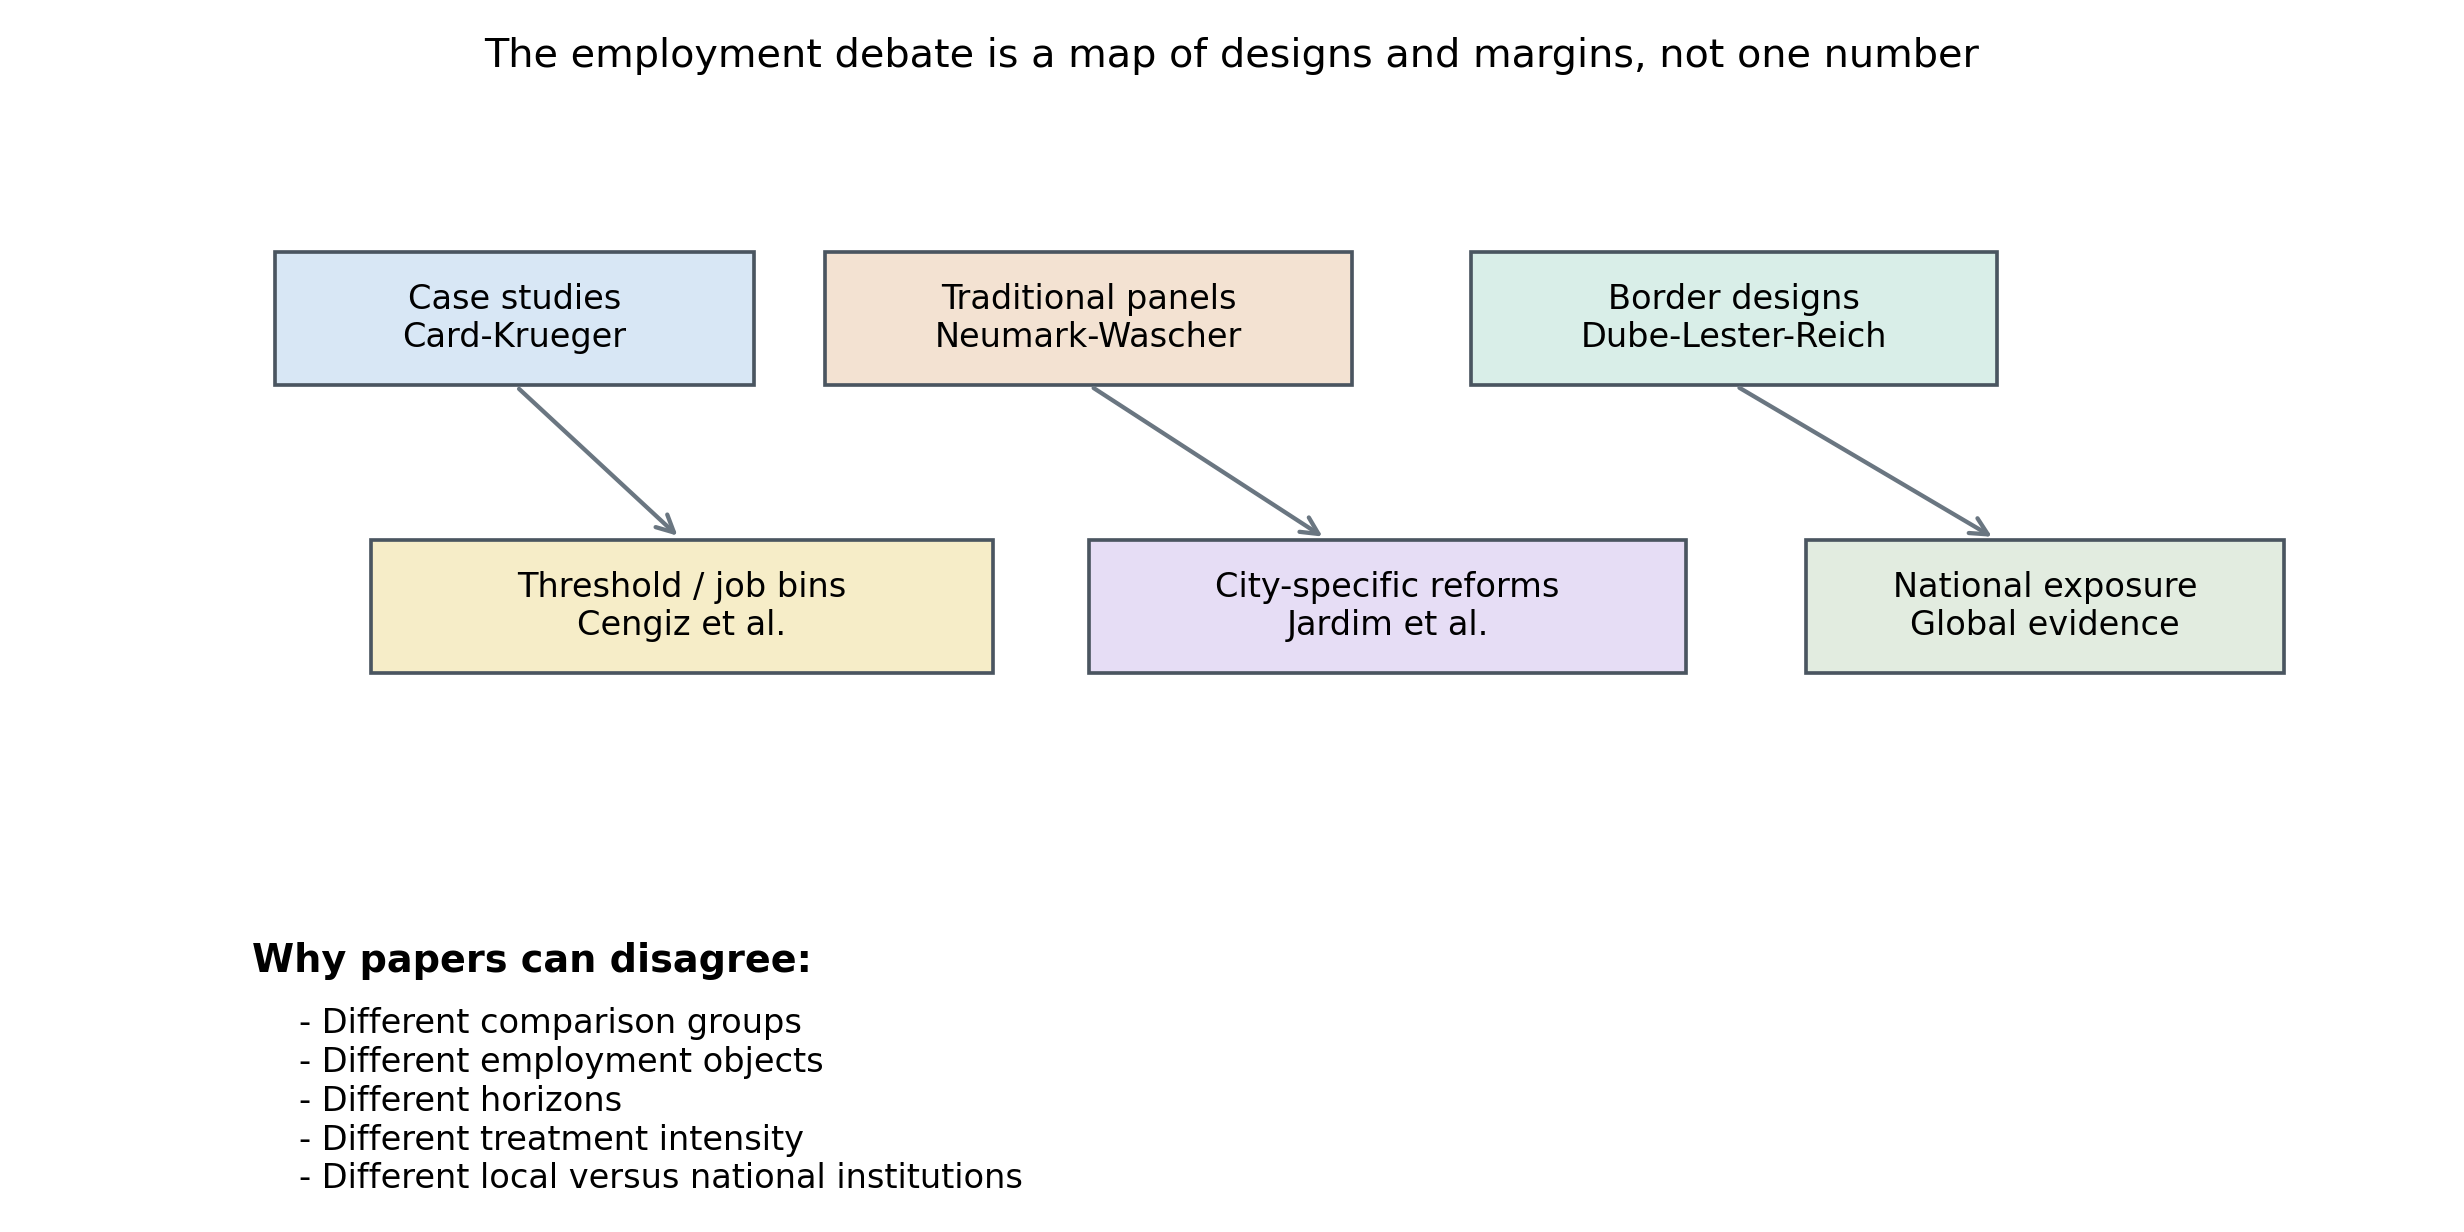
\includegraphics[height=0.72\textheight]{07-employment-debate-landscape.png}
\end{center}
\end{frame}

\begin{frame}{Why papers can disagree without studying different policies}
\small
\begin{tabular}{p{0.2\linewidth} p{0.23\linewidth} p{0.2\linewidth} p{0.26\linewidth}}
\toprule
Design & Unit & Margin observed & Main latent object \\
\midrule
Case study & Establishment & Sector jobs & Untreated local counterfactual \\
Border design & County pair & Local employment, wages & Remaining local shocks \\
Event study & Region-time & Dynamic jobs, hours, prices & Parallel-trends path \\
Wage bins & State-bin panel & Jobs below and above floor & Reclassification versus net jobs \\
National exposure & Worker / firm / region & Wages, inequality, reallocation & Untreated exposure path \\
\bottomrule
\end{tabular}
\end{frame}

\begin{frame}{Modern evidence: separate the margins}
\begin{itemize}
    \item Wages: robust gains and compression near the floor.
    \item Jobs: low-wage job counts may fall even when total employment barely moves.
    \item Hours: intensive-margin cuts can matter, especially after large local hikes.
    \item Turnover and hiring: higher wages can reduce quits but raise screening standards.
    \item Reallocation: some adjustment occurs through firm exit, entry, and worker sorting.
\end{itemize}
\end{frame}

\begin{frame}{Adjustment margins under wage floors}
\begin{center}
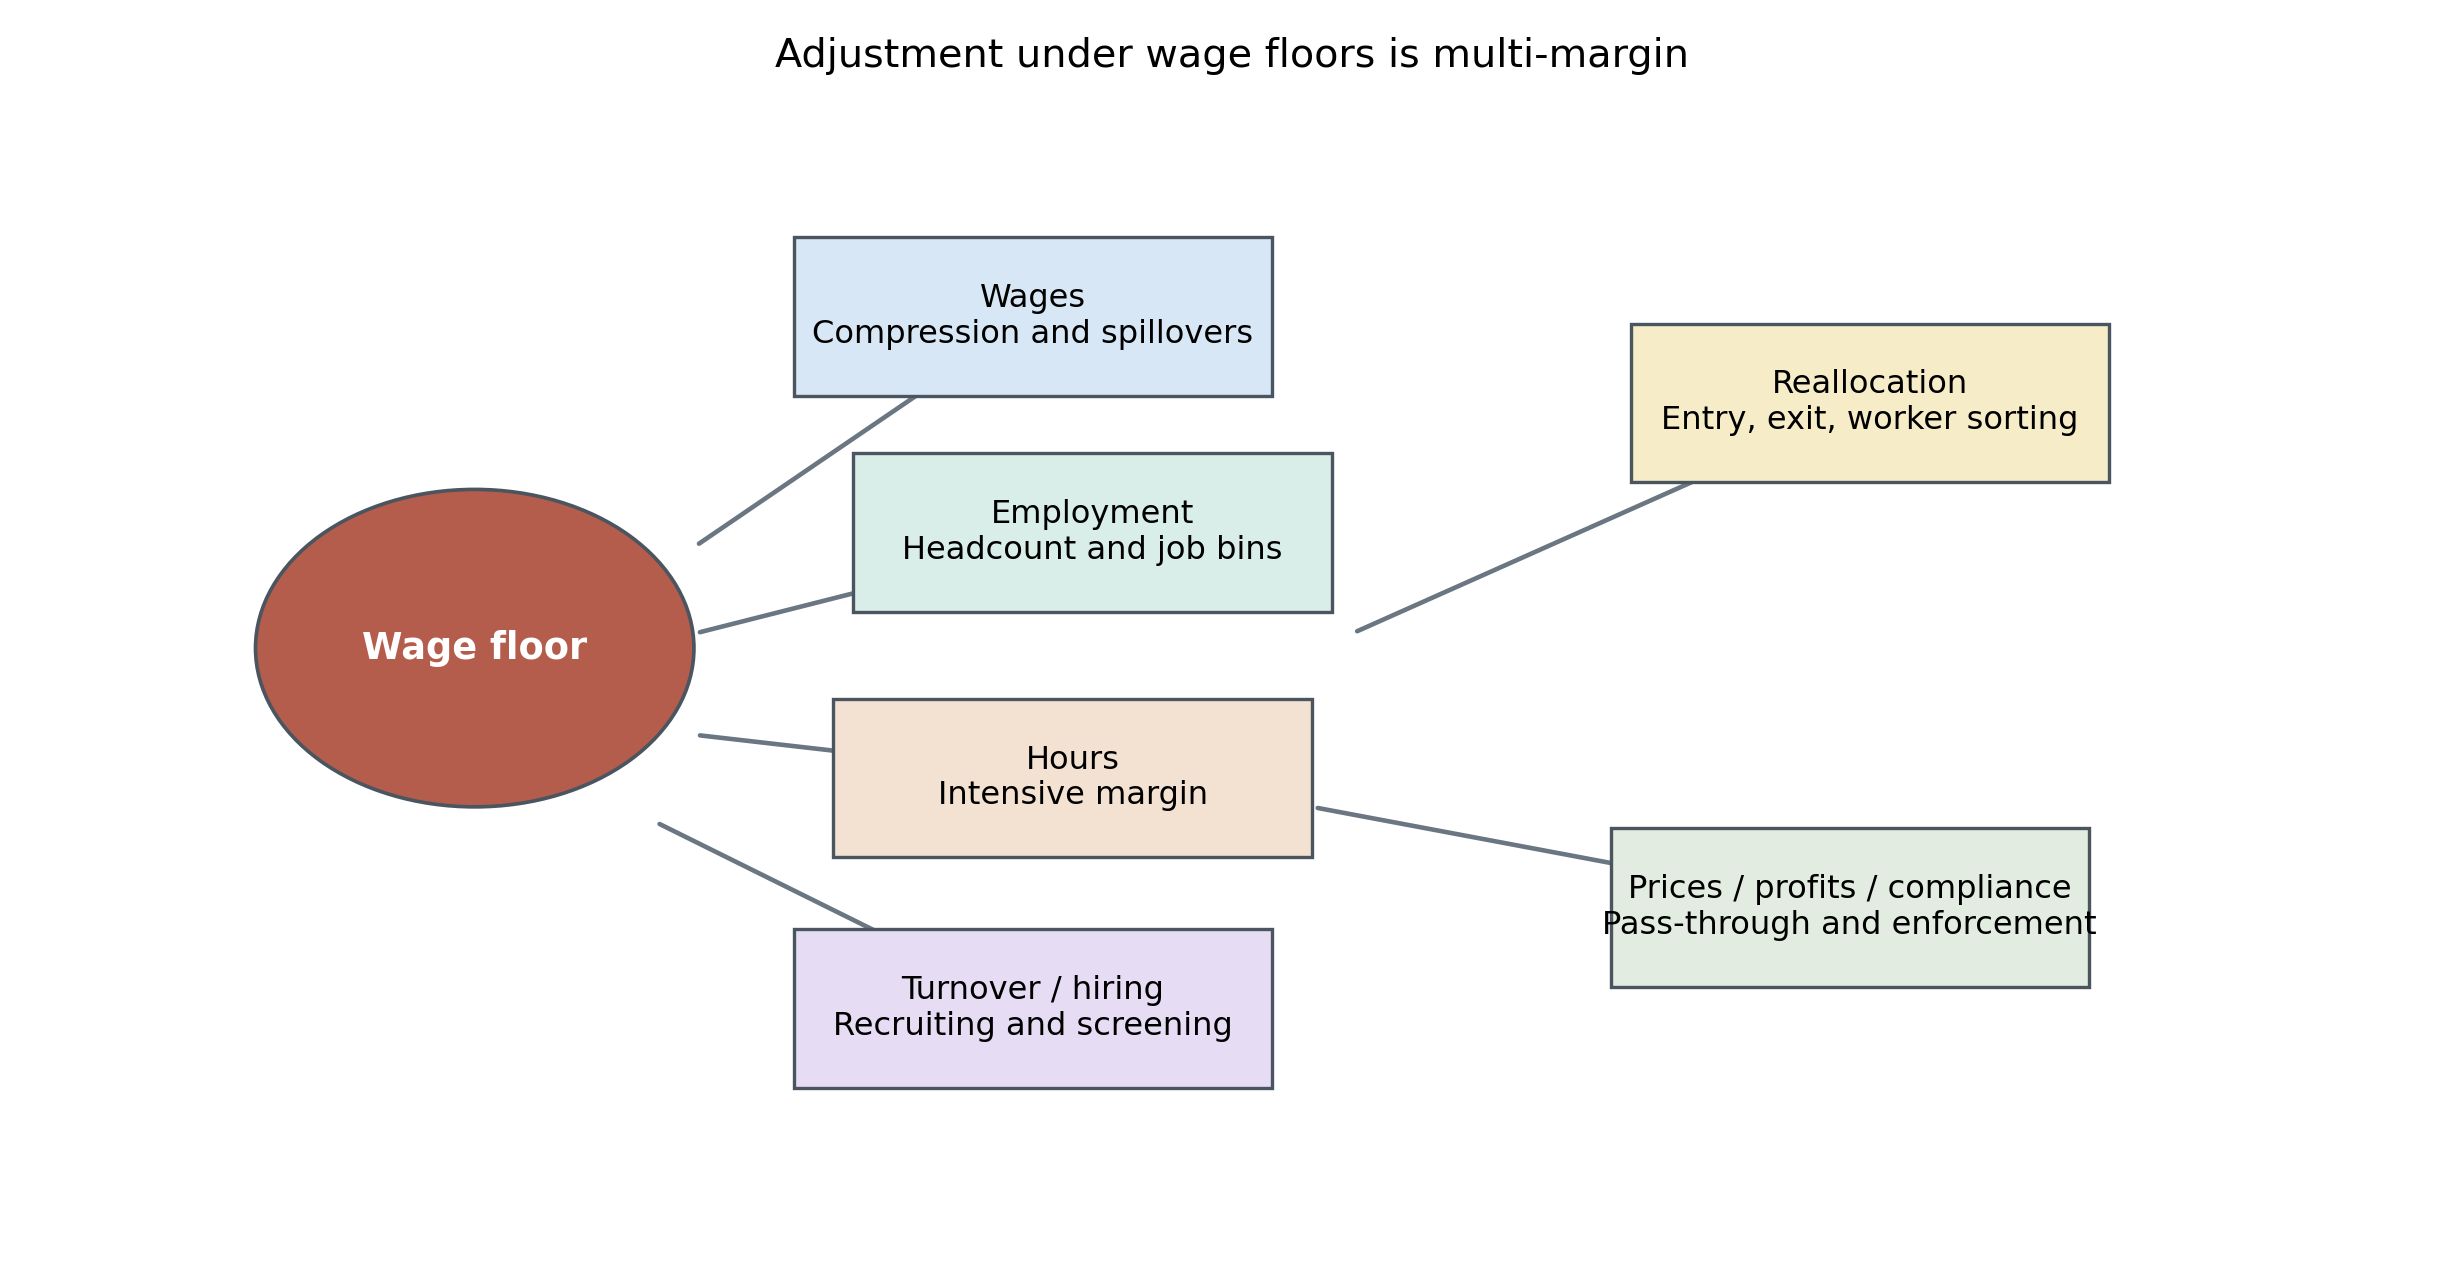
\includegraphics[height=0.72\textheight]{07-adjustment-margins-under-wage-floors.png}
\end{center}
\end{frame}

\begin{frame}{Global evidence}
\begin{itemize}
    \item United States: staggered local and state policy changes, strong wage effects, debate over jobs, hours, and design.
    \item Germany / Europe: national or broad formal-sector reforms, more focus on reallocation, prices, and composition.
    \item Latin America / emerging markets: informality, compliance, and distributional incidence become central.
    \item Global evidence is about institutional heterogeneity, not just more estimates.
\end{itemize}
\end{frame}

\begin{frame}{Global map}
\begin{center}
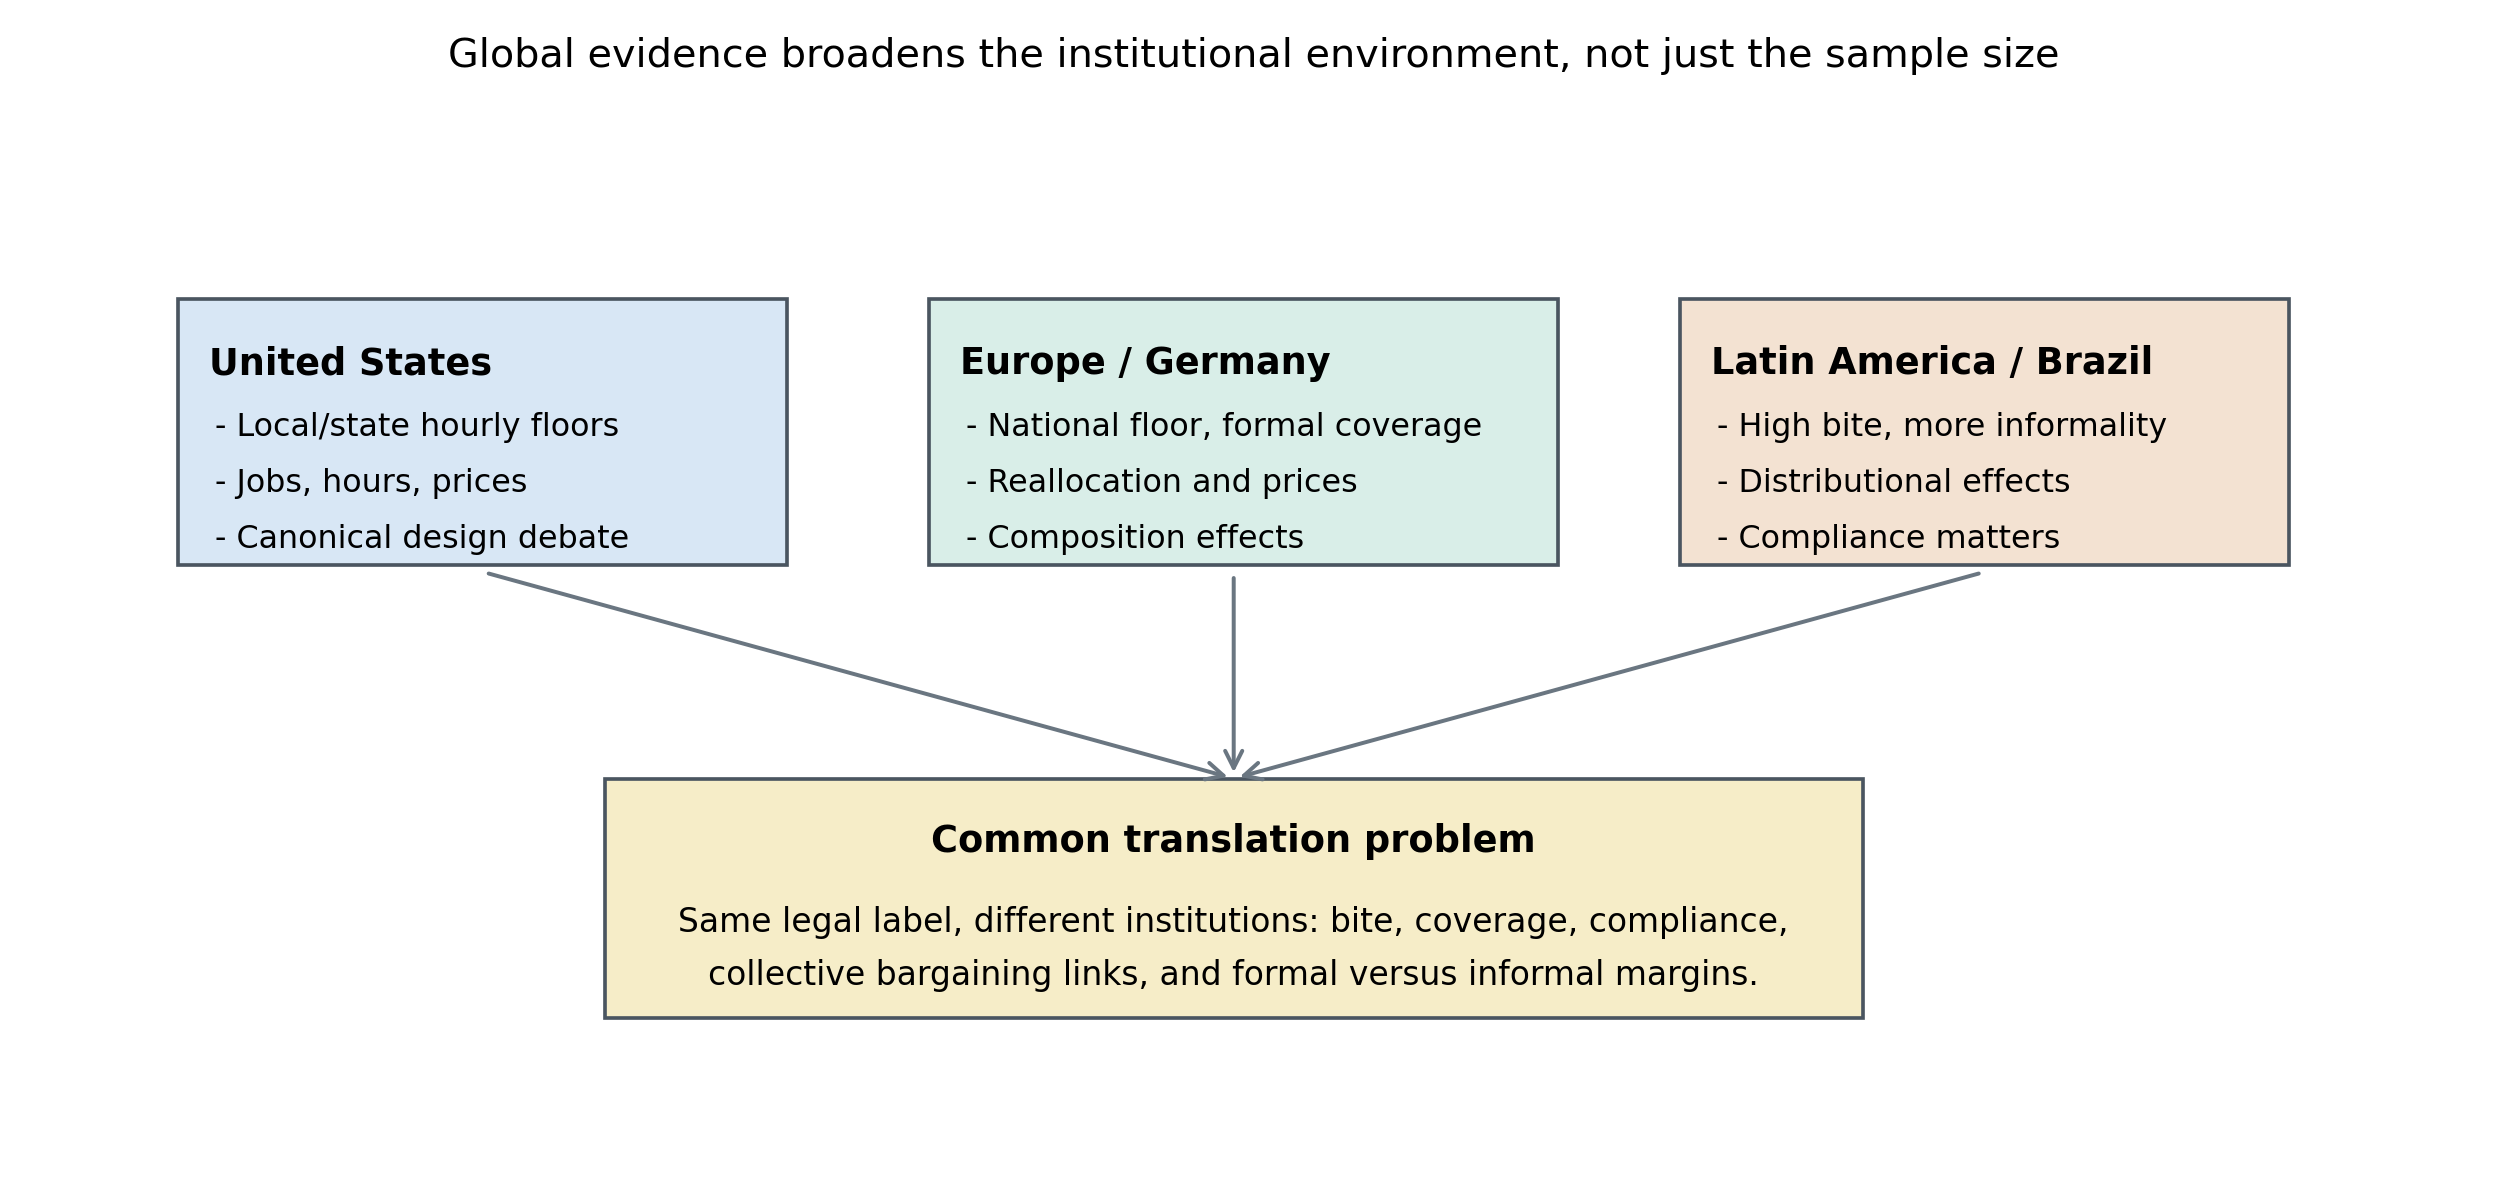
\includegraphics[height=0.72\textheight]{07-global-minimum-wage-evidence-map.png}
\end{center}
\end{frame}

\begin{frame}{Wage law beyond minimum wages}
\begin{itemize}
    \item Minimum wage: direct legal floor on pay.
    \item Enforcement and inspections: whether the legal rule actually binds in practice.
    \item Pay transparency: information shock to bargaining and wage-setting.
    \item Equal-pay rules: restrictions on within-firm pay differentials for similar work.
    \item Keep the object straight: each rule targets a different wage-setting friction.
\end{itemize}
\end{frame}

\begin{frame}{Wage-law toolkit}
\begin{center}
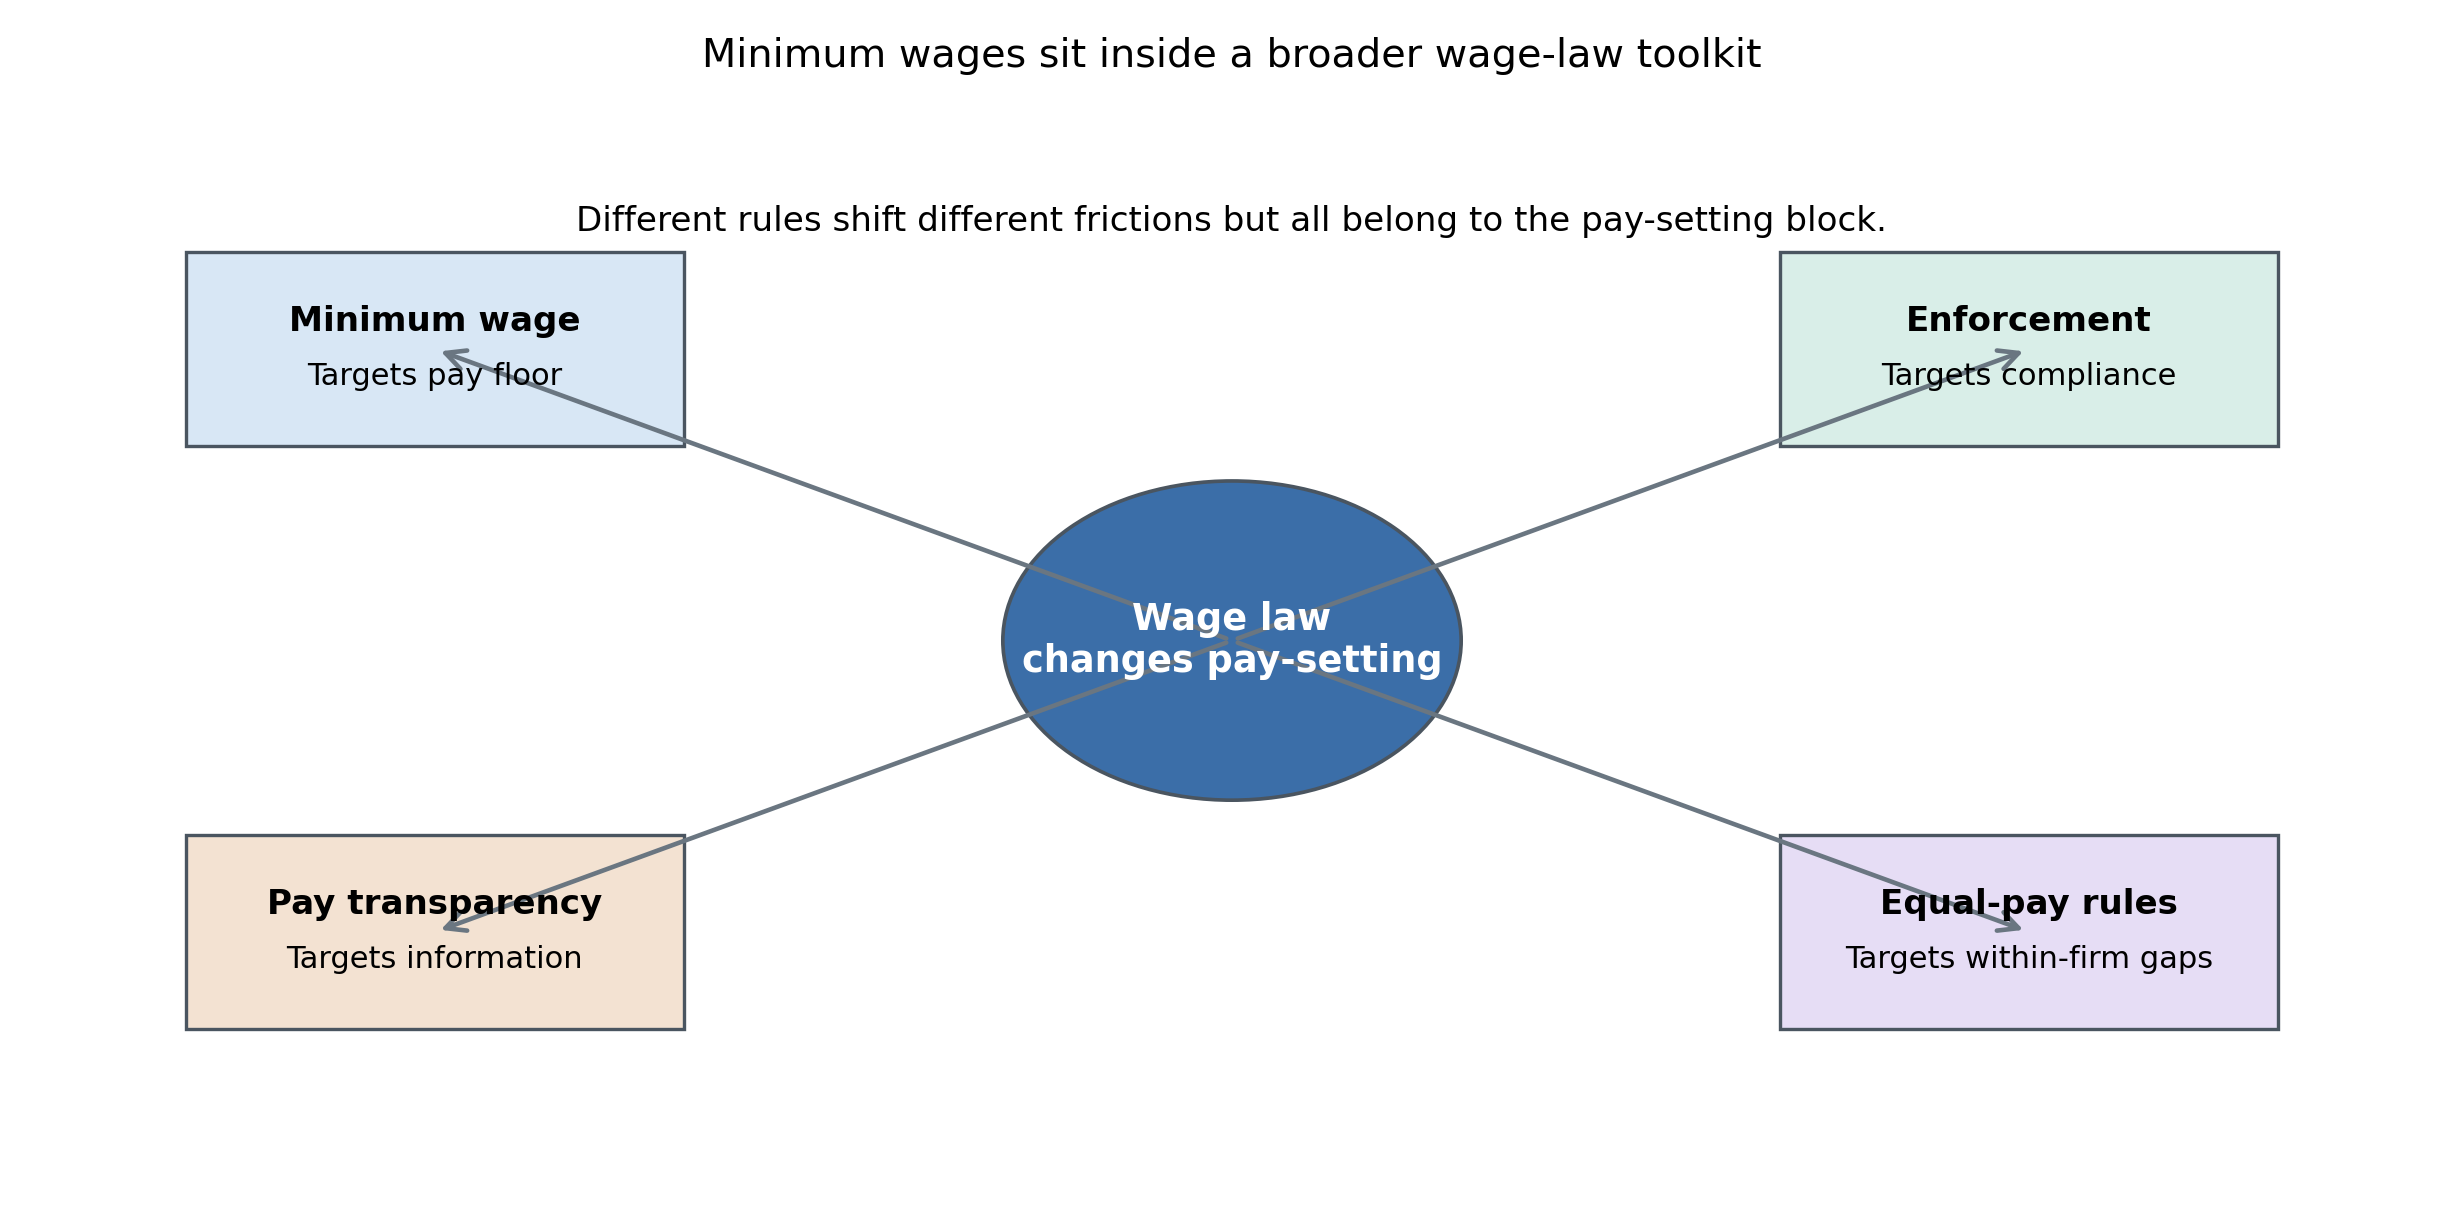
\includegraphics[height=0.72\textheight]{07-wage-law-toolkit.png}
\end{center}
\end{frame}

\begin{frame}{Empirical designs and what they identify}
\begin{itemize}
    \item Border or local comparison designs: policy variation across nearby markets; local wages and employment; remaining local confounds.
    \item Stacked event studies: treatment timing across regions; dynamic outcomes; pre-trend risk.
    \item Threshold-based job-distribution designs: wage bins around the floor; low-wage job counts; spillover and relabeling issues.
    \item National exposure designs: heterogeneous bite across workers or firms; wages, inequality, reallocation; exposure endogeneity.
    \item Enforcement and disclosure designs: inspections or rules; compliance and wage compression; measurement changes alongside behavior.
\end{itemize}
\end{frame}

\begin{frame}{Treatment intensity and compliance}
\[
K_{rt} = \frac{\bar w_{rt}}{\operatorname{median}(w_{rt})}
\]

\[
w_{it}^{obs} = (1-\theta_{it}) w_{it}^{rule} + \theta_{it} w_{it}^{noncomp}
\]

\begin{itemize}
    \item The nominal increase is not the same thing as policy bite.
    \item Observed incidence can differ from legal incidence when compliance is incomplete.
\end{itemize}
\end{frame}

\begin{frame}{Frontier extension}
\begin{itemize}
    \item Link minimum-wage evidence to own-wage elasticities and monopsony measures.
    \item Track spillovers above the floor, not only the exact threshold.
    \item Measure hiring standards, automation, and worker-firm reallocation.
    \item Compare local hikes with national reforms.
    \item Use new worker-firm and compliance data to connect wage law to sorting.
\end{itemize}
\end{frame}

\begin{frame}{Bridge to Week 8}
\begin{itemize}
    \item Week 7 studied legal wage floors and adjacent wage laws.
    \item Week 8 asks what changes when wage determination is mediated by unions, bargaining structures, and worker voice.
    \item The transition question is how decentralized legal rules interact with collective institutions.
\end{itemize}
\end{frame}

\begin{frame}{Takeaways}
\begin{itemize}
    \item Minimum wages test labor-market structure, not only labor-demand slope.
    \item The modern literature separates wages, jobs, hours, turnover, and reallocation.
    \item Different designs can disagree because they identify different margins under different institutions.
    \item Wage law extends beyond minimum wages to enforcement, transparency, and equal-pay rules.
\end{itemize}
\end{frame}

\appendix

\begin{frame}{Appendix: lab bridge}
\begin{itemize}
    \item Reproduce: Cengiz-style grouped wage-bin panel.
    \item Diagnose: Dube-Lester-Reich-style border design and what its counterfactual is.
    \item Transfer: optional Engbom-Moser-style national exposure design with bite and reallocation.
    \item Keep the employment object, treatment intensity, and identifying variation separate in every step.
\end{itemize}
\end{frame}

\end{document}
